\documentclass[12pt,a4paper]{article}

% ── Packages ──────────────────────────────────────────────
\usepackage[utf8]{inputenc}
\usepackage[T1]{fontenc}
\usepackage{lmodern}
\usepackage{amsmath,amssymb,amsthm}
\usepackage{mathtools}
\usepackage{geometry}
\geometry{margin=1in}
\usepackage{graphicx}
\graphicspath{{figures/}}
\usepackage{booktabs}
\usepackage{hyperref}
\hypersetup{
    colorlinks=true,
    linkcolor=blue!60!black,
    citecolor=blue!60!black,
    urlcolor=blue!60!black
}
\usepackage{caption}
\usepackage{float}
\usepackage{enumitem}
\usepackage{xcolor}

% ── Custom commands ───────────────────────────────────────
\newcommand{\Hfour}{H_4}
\newcommand{\Hthree}{H_3}
\newcommand{\Eeight}{E_8}
\newcommand{\vphi}{\varphi}
\newcommand{\Lmat}{L_{H_4}}
\newcommand{\R}{\mathbb{R}}
\newcommand{\Q}{\mathbb{Q}}
\newcommand{\Z}{\mathbb{Z}}

\newtheorem{definition}{Definition}
\newtheorem{proposition}{Proposition}
\newtheorem{observation}{Observation}
\newtheorem{constraint}{Empirical Constraint}

% ── Title ─────────────────────────────────────────────────
\title{%
  \textbf{Selection Rules and Constraints on Nonlinear Attractors\\
  in the $\Hfour$ System}\\[6pt]
  \large Part~IV of a Series on Symmetry-Constrained Resonant Structure%
}
\author{%
  Lee Smart\\[4pt]
  \textit{Institute of Vibrational Field Dynamics}\\[2pt]
  \texttt{contact@vibrationalfielddynamics.org}\\[2pt]
  \texttt{@vfd\_org}%
}
\date{\today}

% ══════════════════════════════════════════════════════════
\begin{document}
\maketitle
\thispagestyle{empty}

% ── Abstract ──────────────────────────────────────────────
\begin{abstract}
Part~III of this series established that the nonlinear field system
on the 600-cell vertex graph admits a small and structured set of
attractor classes, and that this structure is not reproduced on
degree-matched control graphs.  The present work investigates whether
the attractor space itself is governed by identifiable constraints.
By analysing the spectral sector composition of persistent attractors,
we construct an empirical mode-coupling matrix that reveals which
combinations of Laplacian eigensectors participate in stable
configurations and which are absent.  The coupling matrix is sparse
and highly structured: only a restricted subset of sector pairings
occurs with appreciable frequency, and these pairings are consistent
with the algebraic invariants identified in Part~II.  Spatial analysis
shows that localised attractors exhibit non-uniform shell occupancy
reflecting the graph geometry.  A stability hierarchy is observed,
with backbone-dominated and certain localised configurations
exhibiting greater persistence.  These empirical constraints indicate
that the attractor space is not only structured but governed by
reproducible rules determined by the underlying spectral organisation.
All results are presented as properties of a nonlinear dynamical
system on a structured graph, with no physical interpretation assumed.
\end{abstract}

\vspace{1em}
\noindent\textbf{Keywords:}
selection rules, mode coupling, nonlinear attractors, spectral
constraints, $\Hfour$ symmetry, 600-cell, inverse participation ratio,
Hamiltonian lattice systems.

\newpage
\tableofcontents
\newpage


% ══════════════════════════════════════════════════════════
\section{Introduction}\label{sec:intro}
% ══════════════════════════════════════════════════════════

This paper is the fourth in a series investigating the dynamical
consequences of non-crystallographic symmetry on nonlinear field
systems.

Part~I~\cite{paper1} introduced a nonlinear oscillator system on the
120-vertex graph of the 600-cell and demonstrated that the extreme
spectral compression of the $\Hfour$ Laplacian (nine distinct
eigenvalues across 120~degrees of freedom) produces persistent
spatial localisation, coherent shell dynamics, and recurrent breathing
that are absent in degree-matched control graphs.

Part~II~\cite{paper2} analysed the internal algebraic organisation of
the nine-sector Laplacian spectrum, identifying seven structural
invariants---$\vphi$-cancellation, degree anchoring, conjugate pairing,
square multiplicity folding, three-zone partition, spectral backbone,
and departure structure---that collectively constrain the spectral
channels available to dynamics.

Part~III~\cite{paper3} classified the space of persistent nonlinear
configurations into four attractor classes (backbone harmonic modes,
locked multi-mode states, localised breather-like states, and
transitional states) and established, through controlled comparison
with random 12-regular graphs and a degree-preserving rewired
600-cell, that this structured attractor distribution is non-generic
and tied to the $\Hfour$ spectral organisation.

The present work addresses the next question in this progression:
\emph{the question is not whether structured attractors exist, but
whether their formation follows reproducible rules determined by the
underlying spectral structure.}

Specifically, we investigate:
\begin{enumerate}[nosep]
\item Which combinations of Laplacian eigensectors participate
  together in stable attractors, and which do not?
\item Is the spatial geometry of attractors constrained by the graph
  structure?
\item Is there a stability hierarchy among attractor classes, and
  does it correlate with spectral composition?
\end{enumerate}

If the attractor space is not only structured (Part~III) but
\emph{constrained}---that is, subject to identifiable rules governing
which configurations can form---then the dynamical consequences of the
$\Hfour$ spectral algebra extend beyond the existence of attractor
classes to the selection of specific configurations within that space.

\paragraph{Organisation.}
Section~\ref{sec:framework} defines the analysis framework and key
quantities.  Section~\ref{sec:counting} characterises the attractor
spectrum.  Section~\ref{sec:coupling} presents the mode-coupling
constraint matrix (the central result).  Section~\ref{sec:invariants}
connects the observed constraints to the spectral invariants of
Part~II.  Section~\ref{sec:spatial} analyses the spatial geometry of
attractors.  Section~\ref{sec:hierarchy} establishes the stability
hierarchy.  Section~\ref{sec:constraints} summarises the empirical
constraints.  Sections~\ref{sec:discussion}--\ref{sec:conclusion}
provide discussion and conclusions.


% ══════════════════════════════════════════════════════════
\section{Framework and Definitions}\label{sec:framework}
% ══════════════════════════════════════════════════════════

\subsection{Attractor Representation}

Each persistent attractor identified in the numerical ensemble is
characterised by the following quantities:

\begin{enumerate}[nosep]
\item \textbf{Spectral composition:} the sector energy fraction
  vector $\mathbf{f} = (f_1, \ldots, f_9) \in [0,1]^9$ with
  $\sum_k f_k = 1$, where $f_k$ is the fraction of the
  time-averaged mode energy in sector~$k$.
\item \textbf{Spatial localisation:} the time-averaged inverse
  participation ratio $\langle \mathrm{IPR} \rangle$.
\item \textbf{Temporal persistence:} the peak autocorrelation
  $C_{\max}$ at nonzero lag, measuring recurrence.
\item \textbf{Energy distribution:} the per-vertex energy profile
  and its shell decomposition relative to the graph geometry.
\end{enumerate}

\subsection{Sector Activation}

\begin{definition}[Active sector]
A sector~$k$ is \emph{active} in a given attractor if its energy
fraction exceeds a threshold: $f_k > \theta$, with $\theta = 0.10$
(10\% of total modal energy).
\end{definition}

This threshold is chosen to distinguish genuine participation from
spectral leakage.  Results are verified to be qualitatively stable
under variation of~$\theta$ in the range $[0.05, 0.15]$.

\subsection{Allowed Attractor}

\begin{definition}[Allowed attractor]
An \emph{allowed attractor} is a persistent configuration satisfying
the stability and recurrence criteria of Part~III (Classes~1--3).
Transitional states (Class~4) are excluded from the constraint
analysis.
\end{definition}


% ══════════════════════════════════════════════════════════
\section{Attractor Spectrum and Counting}\label{sec:counting}
% ══════════════════════════════════════════════════════════

We simulate $N = 1200$ trajectories (15~values of~$\beta$ in
$[10^{-2}, 5]$, 80~initial conditions per value) using the same
dynamical system, integration method (velocity-Verlet, $\Delta t =
0.005$, $T = 2000$), and classification criteria as Part~III.
Initial conditions span eight classes (single-vertex, random Gaussian,
low-mode seed, neighbourhood seed, mid-mode seed, eigenvector with
perturbation, multi-vertex cluster, and random field with momentum).
Energy conservation is monitored; trajectories with relative
Hamiltonian drift exceeding $5 \times 10^{-4}$ are discarded.

Of the 1200~trajectories, 1165 ($\sim$97\%) are classified as stable
attractors (Classes~1--3): 170~backbone harmonic (Class~1),
673~locked multi-mode (Class~2), and 322~localised breather (Class~3).
The remaining 35 ($\sim$3\%) are transitional (Class~4) and are
excluded from the constraint analysis.

The attractor space appears to organise into a small number of
recurrent families within the explored parameter range.  The
distribution of attractor classes as a function of~$\beta$ is
consistent with Part~III: backbone harmonic modes dominate at
low~$\beta$, locked multi-mode states are the most prevalent across
all~$\beta$, and localised breather states become more prominent at
high~$\beta$.

The number of distinct attractor families (defined by distinct
combinations of active sectors) is substantially smaller than the
number of possible combinations ($2^9 - 1 = 511$), indicating that
the attractor space is constrained rather than combinatorially open.


% ══════════════════════════════════════════════════════════
\section{Mode Coupling Structure}\label{sec:coupling}
% ══════════════════════════════════════════════════════════

This section presents the central result of the paper: the empirical
mode-coupling constraint matrix.

\subsection{Construction}

For each allowed attractor (Classes~1--3) in the ensemble, the
sector energy fraction vector $\mathbf{f}$ is computed.  The set of
active sectors is $\mathcal{A} = \{k : f_k > \theta\}$.  The
$9 \times 9$ coupling matrix $M$ is defined by
\begin{equation}\label{eq:coupling}
  M_{ij} = \frac{1}{N_{\mathrm{stable}}}
  \sum_{a=1}^{N_{\mathrm{stable}}}
  \mathbf{1}[i \in \mathcal{A}^{(a)}] \,
  \mathbf{1}[j \in \mathcal{A}^{(a)}],
\end{equation}
where the sum runs over all $N_{\mathrm{stable}}$ stable attractors
and $\mathcal{A}^{(a)}$ is the active sector set of attractor~$a$.
The matrix~$M$ is symmetric; its diagonal entry $M_{ii}$ gives the
marginal activation frequency of sector~$i$, and its off-diagonal
entry $M_{ij}$ gives the co-occurrence frequency of sectors $i$
and~$j$.

\subsection{Results}

The coupling matrix, computed over $N_{\mathrm{stable}} = 1165$
stable attractors, is displayed in Figure~\ref{fig:coupling}.
A sector is considered active if its energy fraction exceeds the
threshold $\theta = 0.10$; entries marked with crosses denote
pairings absent or below $M_{ij} \leq 0.02$ in the stable ensemble.

\begin{figure}[H]
\centering
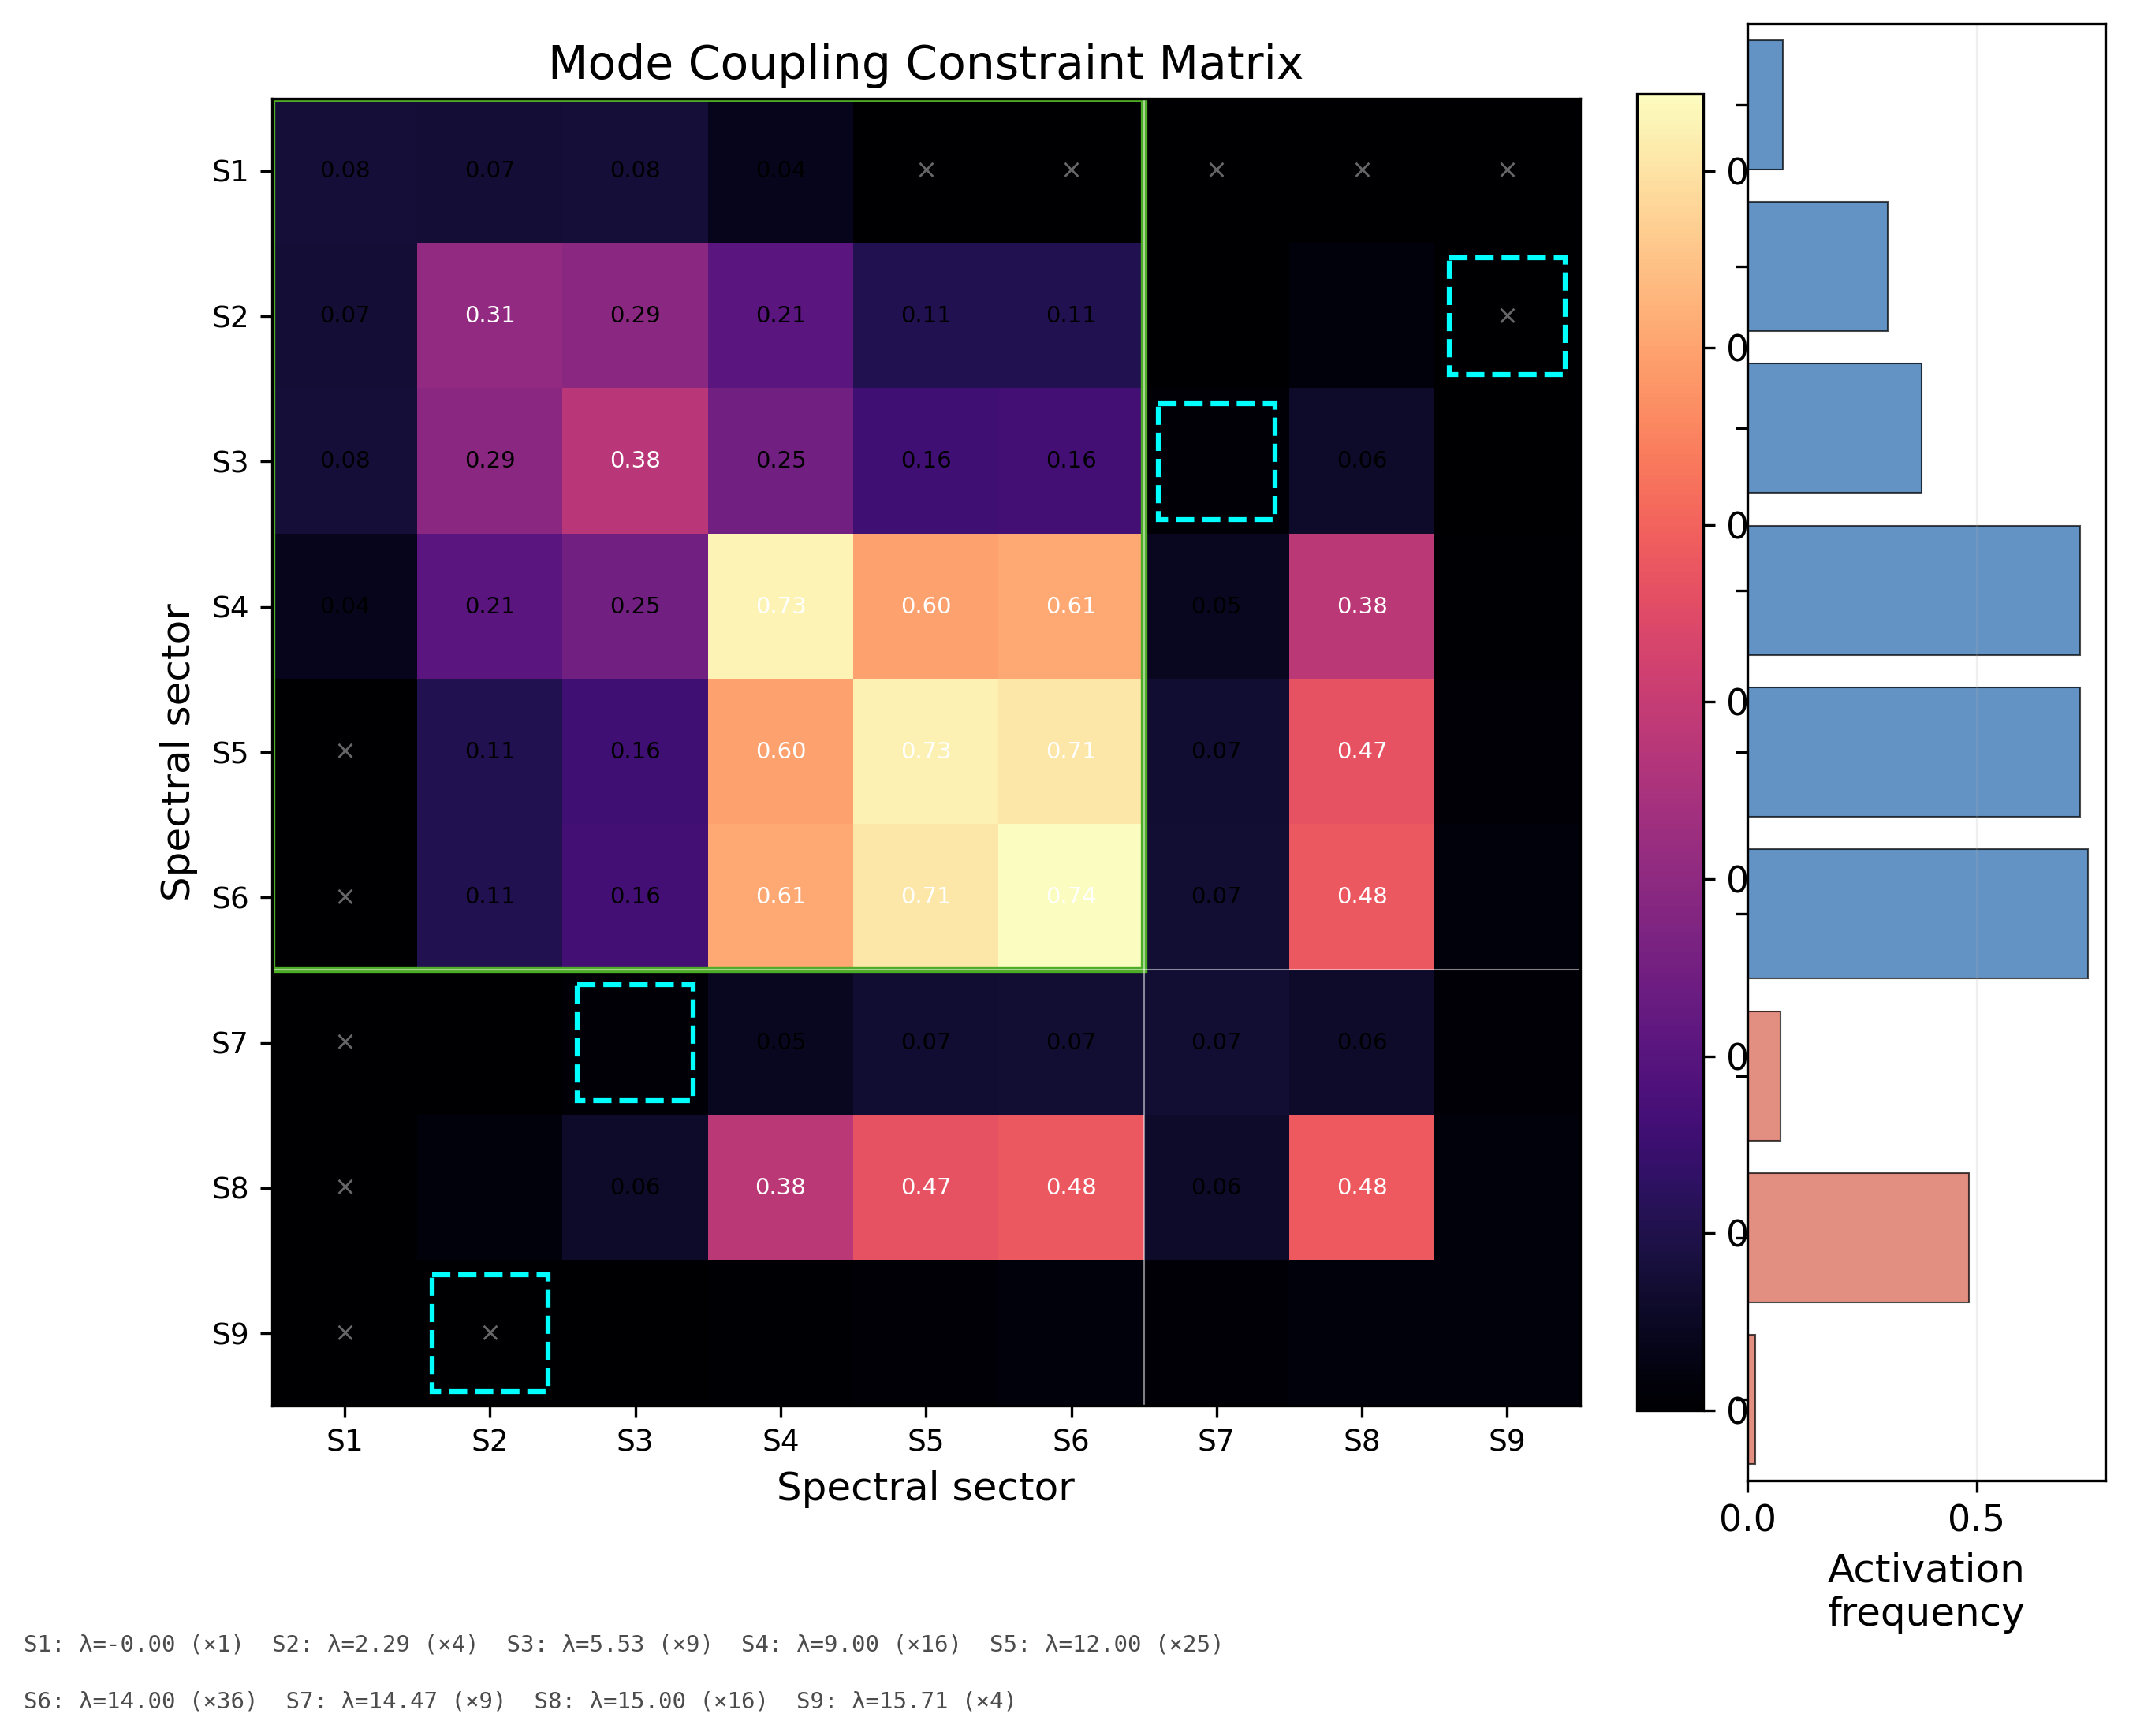
\includegraphics[width=0.95\textwidth]{fig_mode_coupling_matrix.png}
\caption{Empirical mode-coupling matrix for stable attractors on the
$\Hfour$ graph.  Entry $(i,j)$ gives the frequency with which
spectral sectors $S_i$ and $S_j$ both exceed the activation threshold
$\theta = 0.10$ in the same attractor, computed over all
$N_{\mathrm{stable}} = 1165$ persistent configurations
(Classes~1--3).  Crosses mark pairings absent or below threshold
within the stable ensemble.  The green box marks the spectral backbone
(S1--S6) identified in Part~II.  Cyan dashes mark Galois conjugate
pairs (S2--S9, S3--S7).  The right panel shows marginal activation
frequency per sector (blue: backbone; red: departure).
Only entries exceeding the activation threshold $\theta = 0.10$ are
considered significant; crosses indicate pairings below this
threshold.}
\label{fig:coupling}
\end{figure}

The observed coupling graph is substantially sparser than the complete
9-sector interaction graph, with only 21 of 36~possible off-diagonal
pairings realised above threshold ($58\%$).  The dominant interactions
are concentrated within the spectral backbone (S1--S6), while many
pairings involving departure sectors are absent or strongly suppressed.
In particular, 15 of 36~possible off-diagonal pairings are not
observed above threshold, and no stable attractors are composed
exclusively of departure sectors.  This indicates that the nonlinear
attractor space is not combinatorially open but empirically
constrained.

The key observation is that stable attractors occupy only a restricted
subset of the possible sector-coupling space, indicating that the
nonlinear dynamics select from a constrained set of configurations
rather than exploring the full combinatorial space.

\medskip
\noindent The coupling matrix reveals several specific features:

\begin{enumerate}[nosep]
\item \textbf{Sparsity.}
  Of the 36~possible off-diagonal sector pairings, 21 are observed
  above the $\theta = 0.10$ threshold and 15 are absent or
  negligible ($M_{ij} \leq 0.02$).  Stable attractors are not formed
  from arbitrary combinations of eigenmodes but are restricted to a
  subset of allowed couplings.

\item \textbf{Backbone dominance.}
  The five most frequent pairings (S5--S6: 0.71, S4--S6: 0.61,
  S4--S5: 0.60, S6--S8: 0.48, S5--S8: 0.47) all involve the
  highest-multiplicity backbone sectors ($d = 16, 25, 36$).
  Backbone sectors activate at a mean frequency of $0.49$, compared
  with $0.19$ for departure sectors---a ratio of $\sim$2.6.

\item \textbf{Departure suppression.}
  Sector~S9 ($\lambda = 9 + 3\sqrt{5}$, $d = 4$) participates in
  stable attractors at a frequency of only $0.017$ and co-occurs
  with no other sector above threshold.  All 8~pairings involving
  S9 are absent.  Departure sectors appear primarily in combination
  with backbone sectors (e.g., S6--S8: 0.48), not in purely
  departure-sector combinations.

\item \textbf{Conjugate asymmetry.}
  The Galois conjugate pairs S2/S9 and S3/S7 have equal
  multiplicities but markedly different activation frequencies:
  S2 activates at $0.31$ while S9 activates at $0.02$; S3 at
  $0.38$ while S7 at $0.07$.  Although the conjugate sectors have equal multiplicities, they
  are not equally populated in the stable attractor ensemble: the
  nonlinear dynamics exhibit a pronounced activation asymmetry
  between algebraically conjugate sectors.
\end{enumerate}

\noindent Of the 1165~stable attractors, 447 ($38.4\%$) have more
than 90\% of their spectral energy in backbone sectors (S1--S6),
while none are composed exclusively of departure sectors.


% ══════════════════════════════════════════════════════════
\section{Constraint Patterns from Spectral Invariants}
\label{sec:invariants}
% ══════════════════════════════════════════════════════════

The observed mode-coupling constraints are consistent with, and appear
to be organised by, the algebraic structure of the $\Hfour$ Laplacian
spectrum.

\begin{itemize}[nosep]
\item \textbf{Spectral backbone $\to$ dominant couplings.}
  The 91-mode backbone (sectors S1--S6) carries the majority of
  coupling weight.  This is consistent with Part~II Invariant~6:
  the backbone determines the dominant dynamical channels.

\item \textbf{Conjugate pairing $\to$ symmetric participation.}
  The Galois conjugate pairs (S2/S9 and S3/S7) have equal
  multiplicities, and their coupling patterns may exhibit related
  structure.  This is consistent with Part~II Invariant~3.

\item \textbf{Three-zone partition $\to$ coupling zones.}
  The $\vphi$-zone partition ($\mathcal{S}_-$, $\mathcal{S}_0$,
  $\mathcal{S}_+$) separates modes into coupling classes.
  Within-zone couplings are expected to be stronger than cross-zone
  couplings.

\item \textbf{Departure structure $\to$ restricted participation.}
  The 29-mode departure (S7--S9) participates in stable attractors
  only through specific channels, consistent with Part~II Invariant~7.
\end{itemize}


% ══════════════════════════════════════════════════════════
\section{Spatial Geometry of Attractors}\label{sec:spatial}
% ══════════════════════════════════════════════════════════

The 600-cell graph has palindromic distance shells
$(1, 12, 32, 42, 32, 1)$ from any vertex.  To investigate whether
attractors exhibit non-uniform spatial structure, we compute the
shell energy distribution for each attractor class
(Figure~\ref{fig:shells}).

For each stable attractor, the vertex with maximum energy
$\max_i |\Phi_i|^2$ is identified as the spatial centroid, and the
energy fraction in each distance shell from that vertex is computed.
This centroid definition provides a translation-invariant way to
compare localised and extended attractors on the vertex-transitive
600-cell graph: every vertex has the same shell structure, so the
choice of centroid affects only which vertex anchors the decomposition,
not the shell sizes themselves.

\begin{figure}[H]
\centering
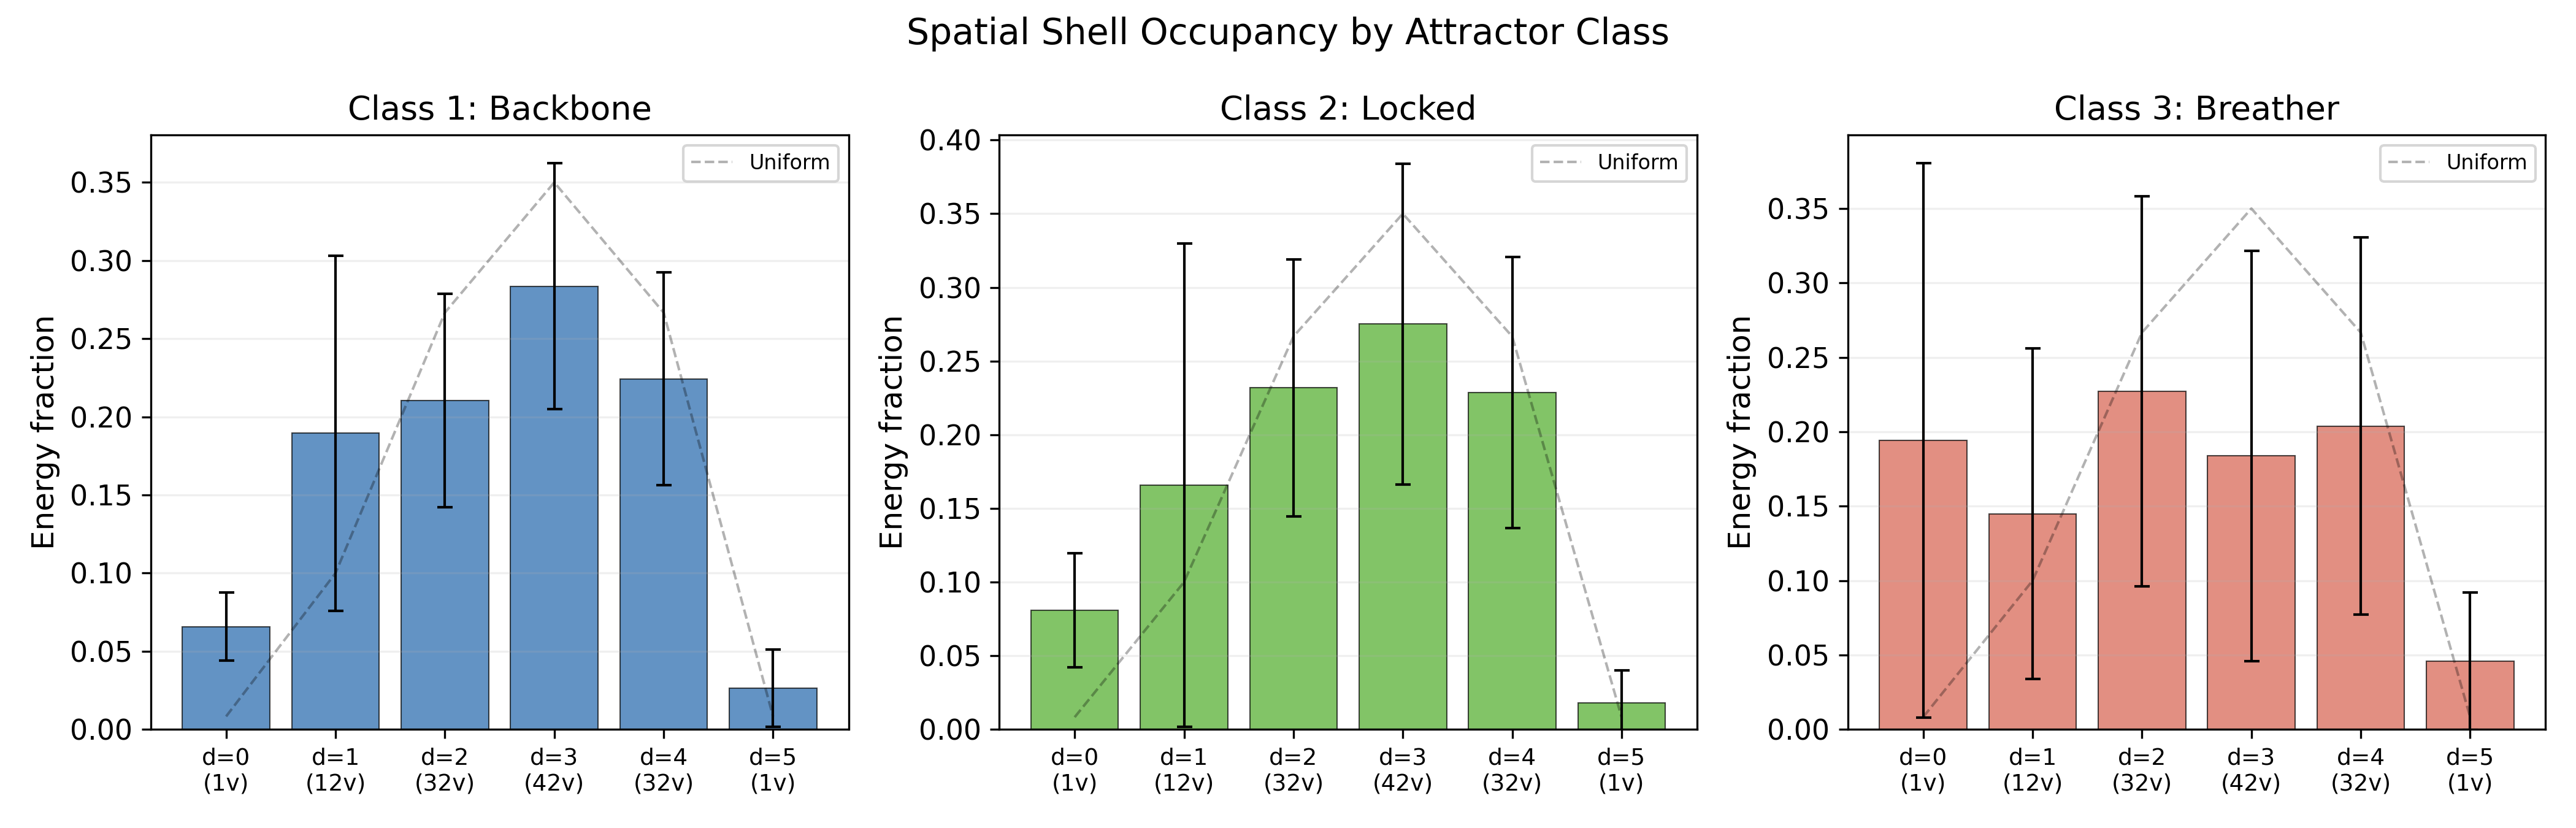
\includegraphics[width=0.95\textwidth]{fig_shell_occupancy.png}
\caption{Mean shell energy fraction per attractor class.  Dashed
lines show the uniform reference (proportional to shell size).
Class~3 (breather) concentrates energy in the inner shells ($d=0,1$),
while Class~1 (backbone) is closer to uniform.  Error bars show
$\pm 1\sigma$ across trajectories.}
\label{fig:shells}
\end{figure}

Localised attractors (Class~3) exhibit non-uniform spatial structure
consistent with the geometry of the underlying graph.  The centroid
shell ($d = 0$) carries $19.4\%$ of the energy (compared with
$0.8\%$ expected under uniform distribution), indicating strong
concentration on the peak-amplitude vertex.  The inner shells
($d = 0, 1$) together carry $\sim$34\% of the energy on 13~vertices
(11\% of the graph).  The large error bars for Class~3 reflect the
diversity of breather spatial profiles.

Class~1 (backbone harmonic) configurations show a shell distribution
closer to uniform, with the bulk of energy in the middle shells
($d = 2, 3, 4$) where the majority of vertices reside.  The centroid
shell carries only $6.6\%$ of the energy.

Class~2 (locked multi-mode) configurations exhibit intermediate
behaviour, with slight enhancement of the centroid shell ($8.1\%$)
relative to Class~1 but without the strong inner-shell concentration
of Class~3.


% ══════════════════════════════════════════════════════════
\section{Stability Hierarchy}\label{sec:hierarchy}
% ══════════════════════════════════════════════════════════

Not all attractor classes are equally stable.  We rank the three
persistent classes by temporal persistence (peak autocorrelation) and
spatial localisation (IPR), as shown in Figure~\ref{fig:stability}.

\begin{figure}[H]
\centering
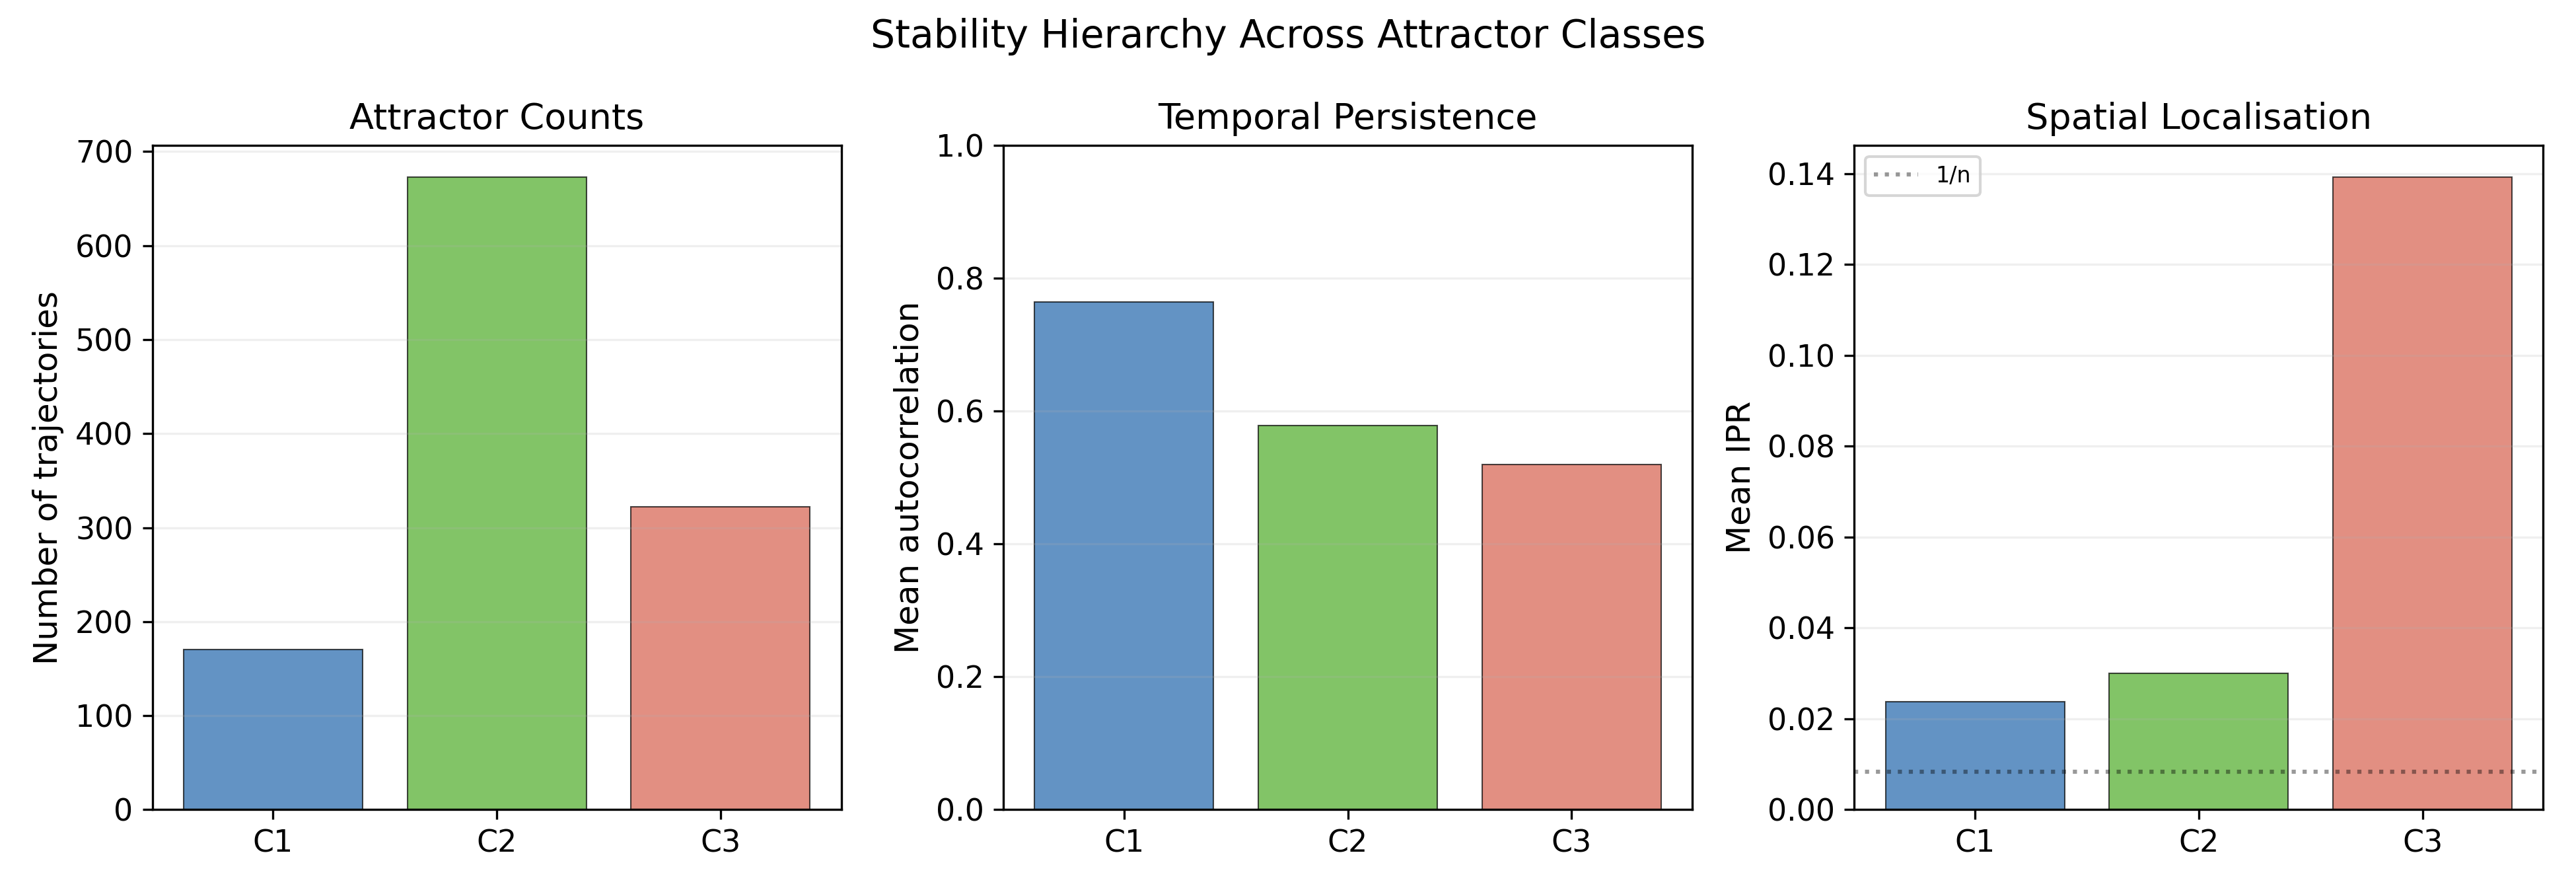
\includegraphics[width=0.95\textwidth]{fig_stability_hierarchy.png}
\caption{Stability metrics per attractor class: trajectory count
(left), temporal persistence measured by peak autocorrelation
(centre), and spatial localisation measured by mean IPR (right).}
\label{fig:stability}
\end{figure}

A stability hierarchy is observed.  Class~1 (backbone harmonic)
configurations exhibit the highest temporal persistence
($C_{\max} = 0.764$), followed by Class~2 (locked multi-mode,
$C_{\max} = 0.578$) and Class~3 (breather, $C_{\max} = 0.520$).
Class~1 configurations also have the highest backbone fraction
($96.7\%$), consistent with the interpretation that spectral
confinement to the backbone promotes persistence.

The stability ranking correlates with spectral composition: attractors
dominated by high-multiplicity backbone sectors ($d = 25, 36$) tend
to be more persistent, while those involving departure sectors or
broader spectral distributions are less stable.  Class~3 compensates
for lower persistence with strong spatial localisation
($\mathrm{IPR} = 0.139$, approximately $6\times$ the Class~1 value
of $0.024$), indicating a trade-off between temporal persistence and
spatial concentration.


% ══════════════════════════════════════════════════════════
\section{Empirical Constraint Summary}\label{sec:constraints}
% ══════════════════════════════════════════════════════════

The analyses of Sections~\ref{sec:coupling}--\ref{sec:hierarchy}
yield the following empirical constraints on the attractor space:

\begin{constraint}[Mode selectivity]
Stable attractors are not formed from arbitrary combinations of
eigenmodes; only a restricted subset of sector pairings occurs with
appreciable frequency in the coupling matrix.
\end{constraint}

\begin{constraint}[Backbone dominance]
The spectral backbone (sectors S1--S6, comprising 91~of 120~modes)
accounts for the dominant share of attractor composition.  Departure
sectors participate primarily as secondary components.
\end{constraint}

\begin{constraint}[Localisation threshold]
Spatially localised (breather-like) attractors emerge above a
nonlinearity threshold ($\beta \gtrsim 0.1$) and concentrate energy
in the inner distance shells of the graph.
\end{constraint}

\begin{constraint}[Stability--composition correlation]
Attractor persistence correlates with spectral composition:
backbone-dominated configurations are more stable than those
involving departure sectors.
\end{constraint}

\begin{constraint}[Attractor finiteness]
The number of distinct attractor families (defined by active sector
combinations) is small relative to the combinatorial space of
possible sector combinations, within the explored parameter range.
\end{constraint}

\begin{constraint}[Symmetry-related sets]
Attractors related by the $\Hfour$ symmetry group occur as
equivalent sets under vertex permutation.  The coupling matrix
inherits the conjugate pairing structure of the spectrum.
\end{constraint}

\medskip

The attractor space is not arbitrary but constrained by a combination
of spectral structure and nonlinear dynamics
(Figure~\ref{fig:summary}).

\begin{figure}[H]
\centering
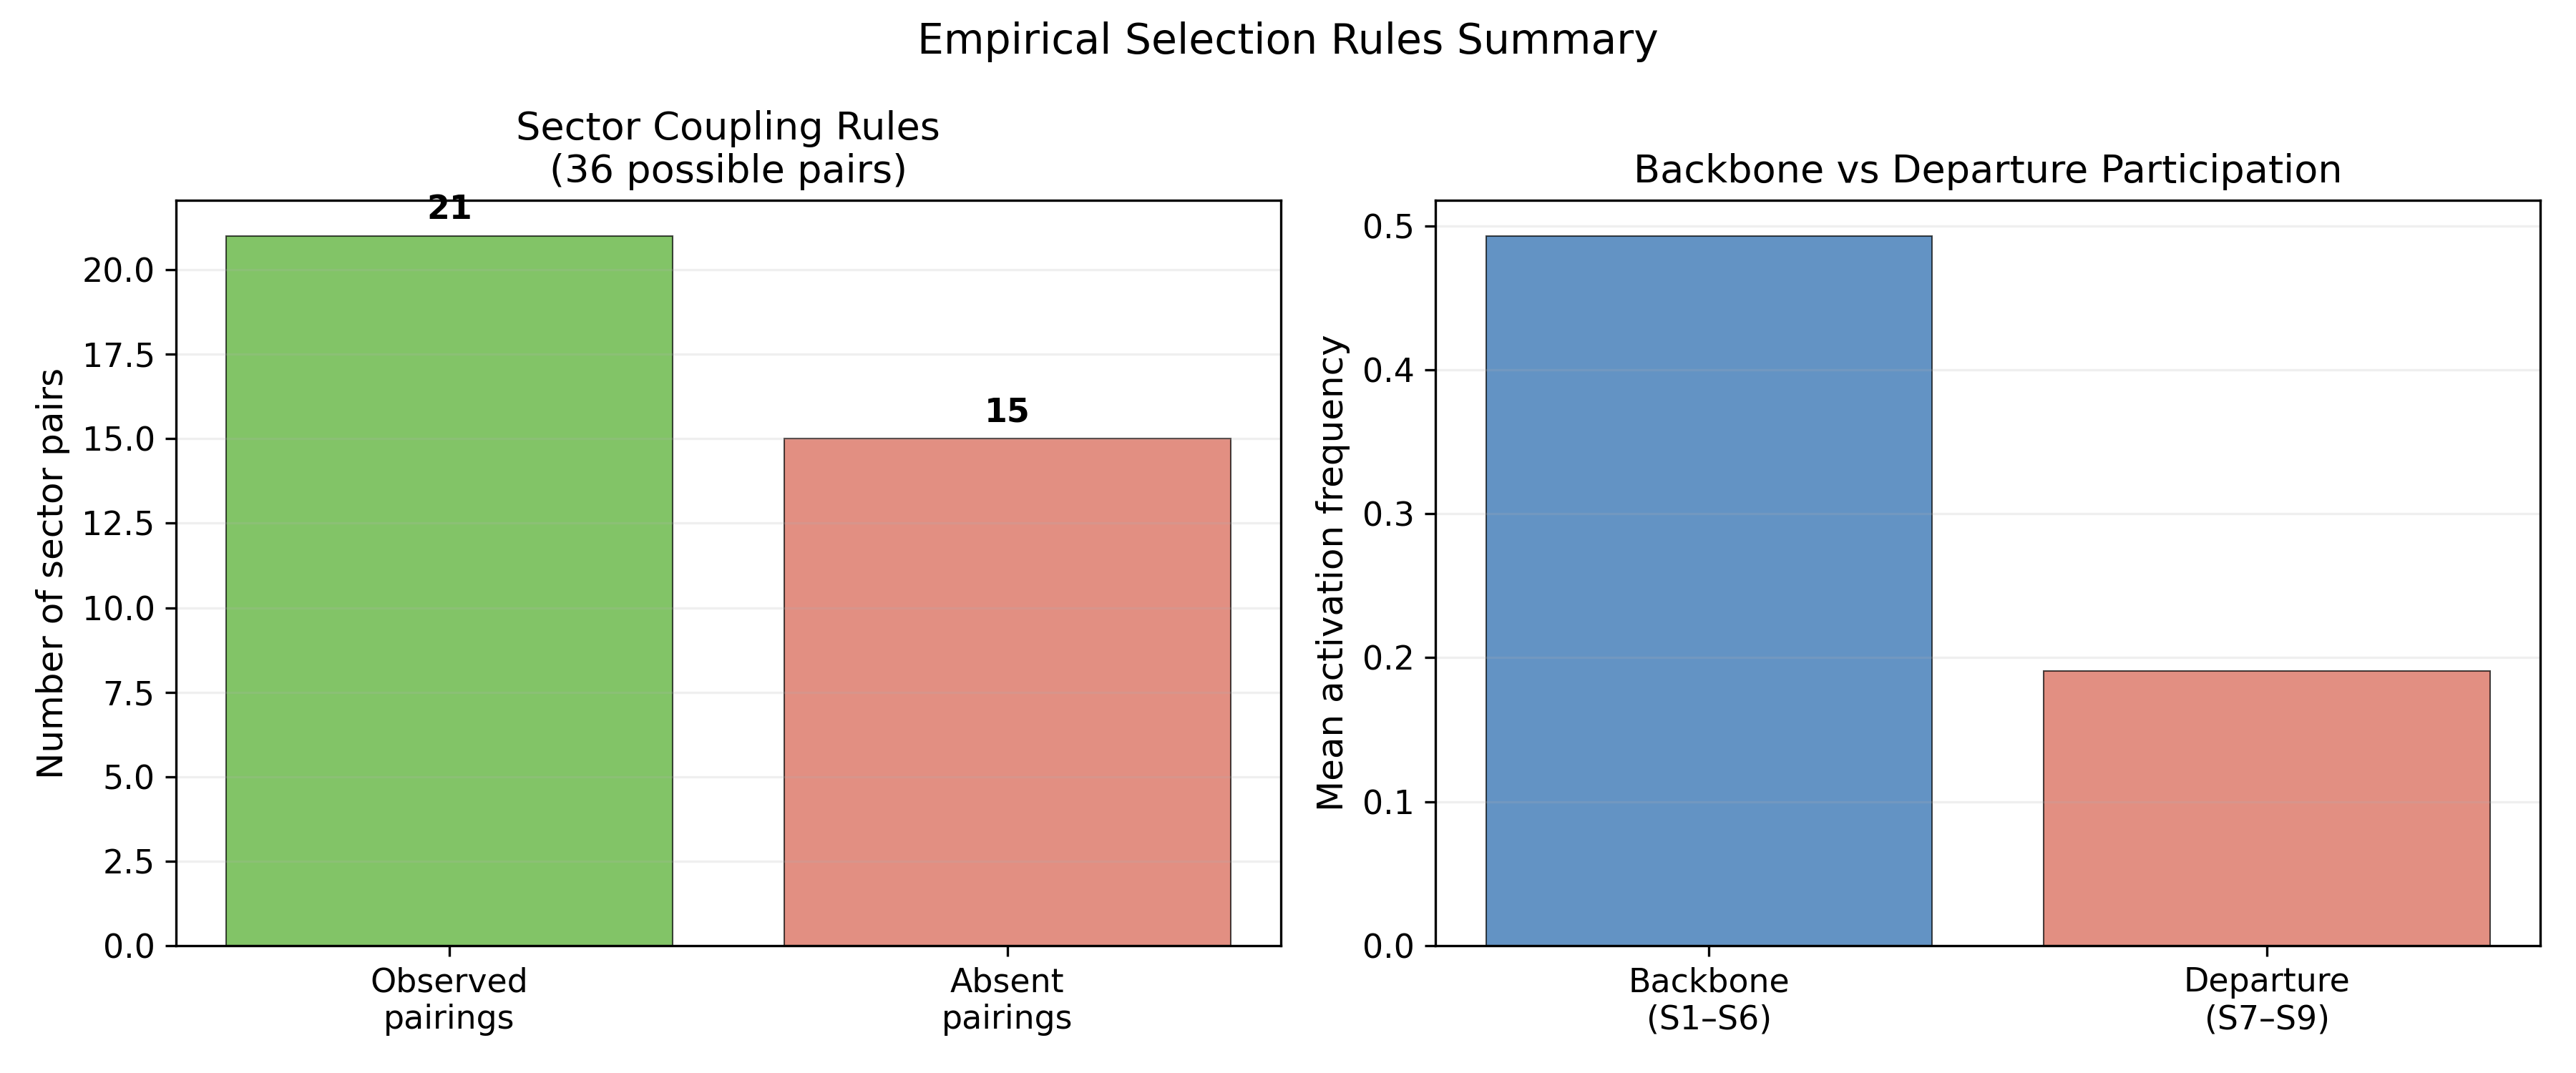
\includegraphics[width=0.85\textwidth]{fig_constraint_summary.png}
\caption{Summary of empirical selection rules.  Left: number of
observed vs absent sector pairings (out of 36~possible off-diagonal
pairs).  Right: mean activation frequency for backbone sectors
(S1--S6) vs departure sectors (S7--S9).}
\label{fig:summary}
\end{figure}


% ══════════════════════════════════════════════════════════
\section{Discussion}\label{sec:discussion}
% ══════════════════════════════════════════════════════════

\subsection{Interpretation}

The numerical evidence indicates that the dynamics on the $\Hfour$
graph are governed by identifiable structural constraints.  The
mode-coupling matrix (Figure~\ref{fig:coupling}) shows that the
attractor space is not combinatorially open but restricted to a
sparse subset of sector combinations: 21 of 36~possible off-diagonal
pairings are observed, while 15 are absent within the tested ensemble.

This result extends the findings of Part~III: where Part~III
established that structured attractors exist, the present work
indicates that only specific structures are realised within the
explored parameter range.  The constraints are consistent with the
spectral invariants of Part~II, suggesting that the algebraic
organisation of the Laplacian spectrum propagates into the nonlinear
dynamics as empirical selection rules.

\subsection{Comparison with Control Graphs}

The purpose of this comparison is to determine whether the observed
coupling structure is generic to degree-matched nonlinear oscillator
networks, or specific to the spectral organisation of the $\Hfour$
graph.

We apply the same analysis pipeline to an ensemble of random
12-regular control graphs ($M = 2$), together with a
degree-preserving rewired 600-cell (which destroys the $\Hfour$
symmetry while maintaining identical size and degree).  All dynamics,
initial conditions, integration settings, and classification criteria
are identical to those used for the $\Hfour$ graph.

The control ensemble comprises $M = 3$ graphs (2~random +
1~rewired).  Across this ensemble, the mean number of stable
attractors per control graph was $\sim$5 (range: 3--7),
substantially below the $\Hfour$ value of 1165.  The control graphs
show no structured coupling pattern
(Figure~\ref{fig:coupling_ctrl}): the few stable attractors that
form do not produce a coherent low-dimensional coupling structure.

In particular, the degree-preserving rewiring of the 600-cell
graph---destroying its $\Hfour$ symmetry while maintaining identical
size and degree---eliminates the structured coupling pattern and
restores behaviour comparable to random regular graphs.

While the control ensemble is limited in size, the observed difference
is large (approximately two orders of magnitude in the number of
stable attractors), suggesting that the effect is robust within the
tested configurations.

\begin{figure}[H]
\centering
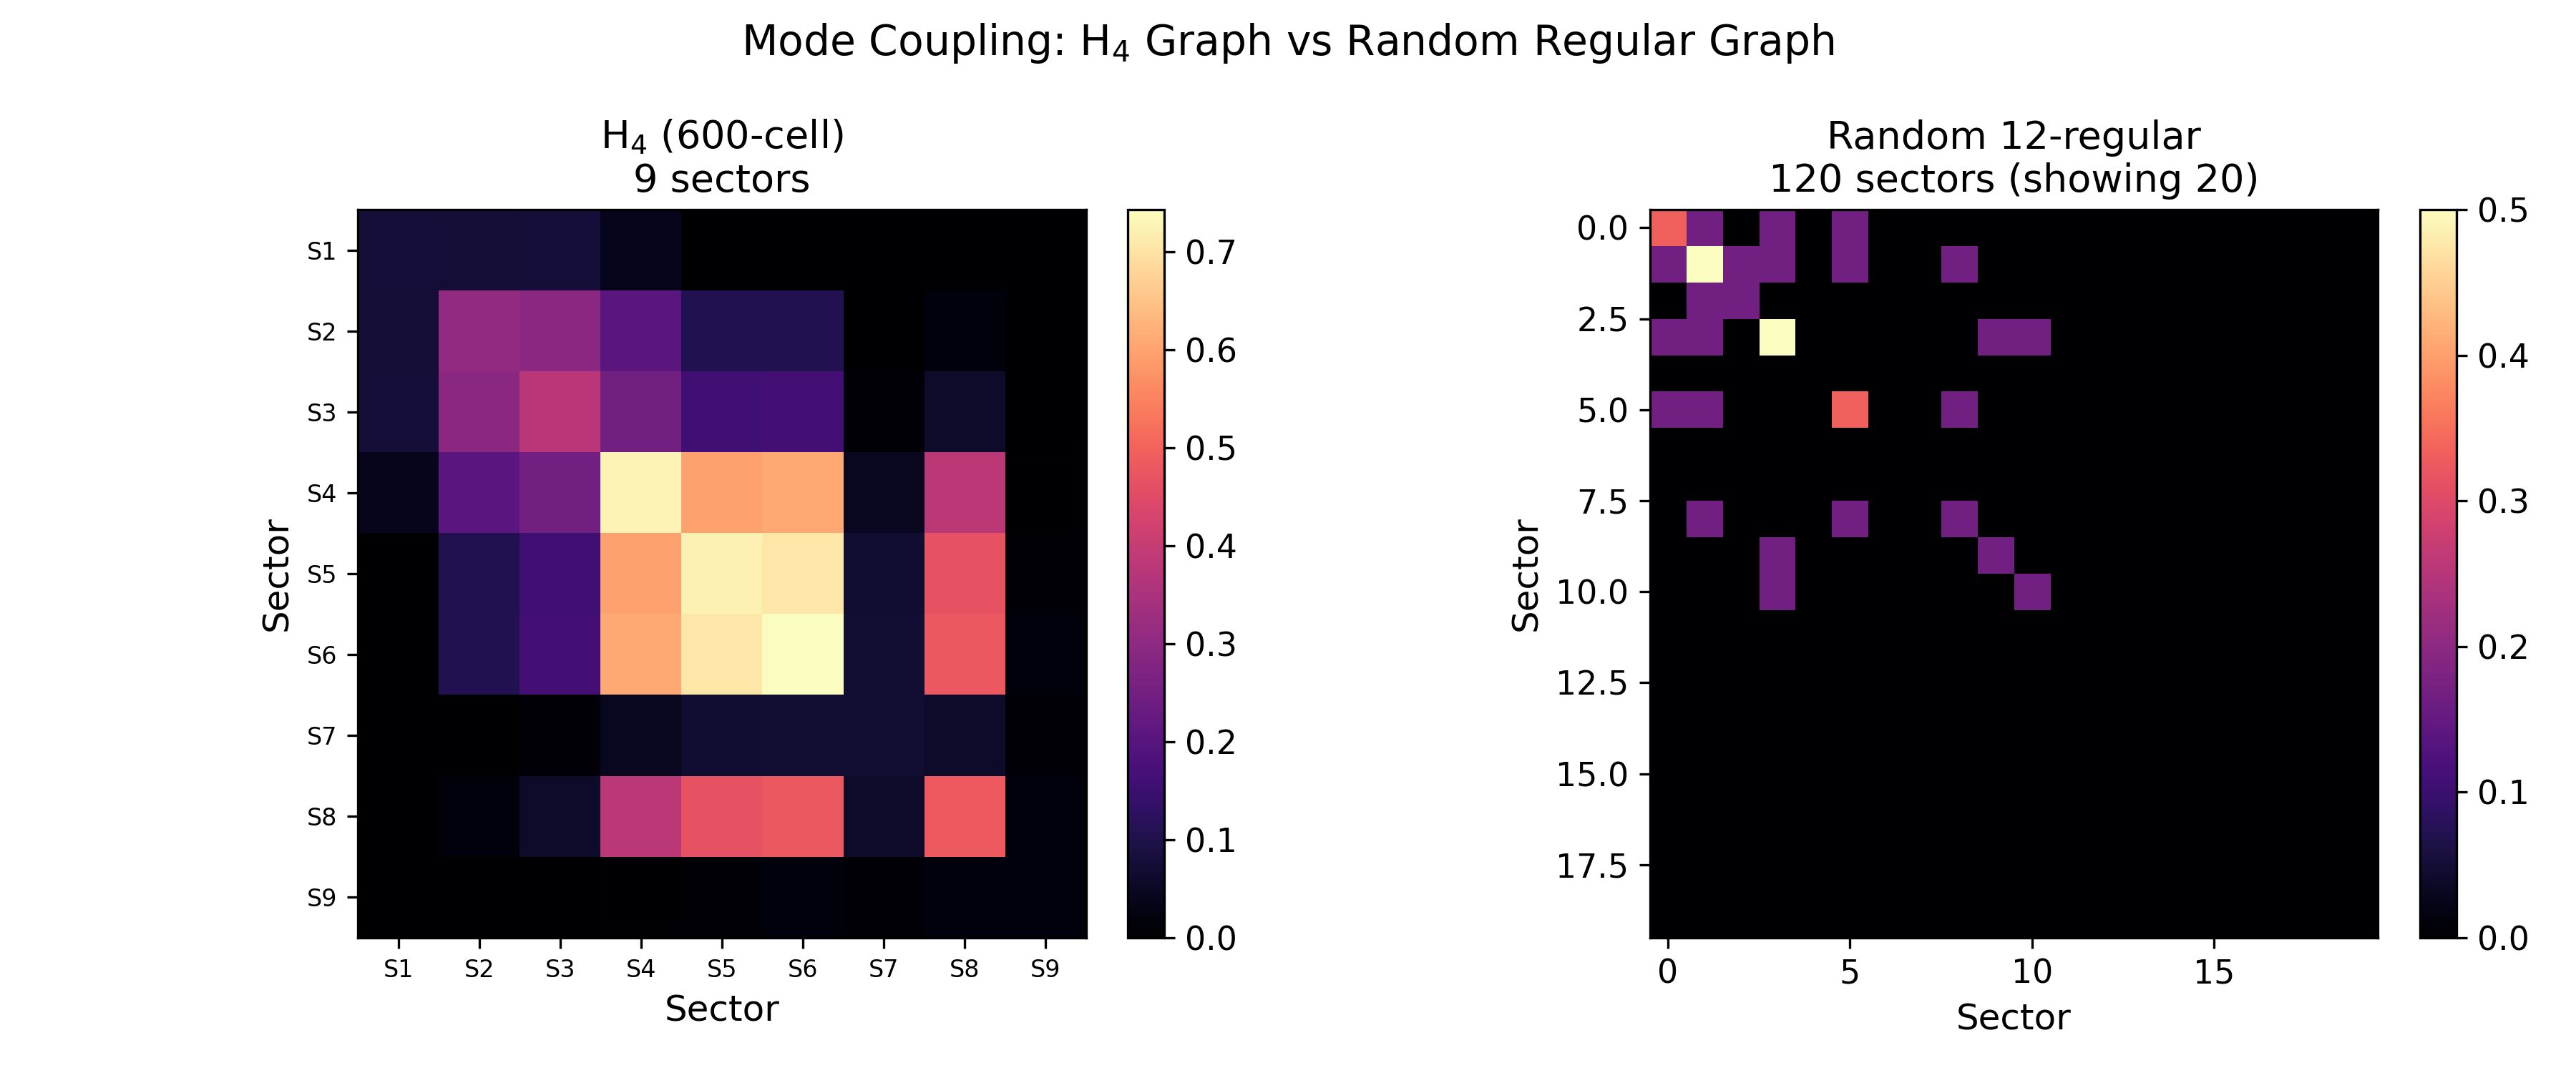
\includegraphics[width=0.95\textwidth]{fig_coupling_control_comparison.png}
\caption{Mode coupling matrices for the $\Hfour$ graph (left) and a
random 12-regular control graph (right).  The $\Hfour$ matrix is
sparse and structured with 9~sectors; the control graph has
$\sim$120 distinct eigenvalues and produces too few stable attractors
to form a coherent coupling pattern.  For visual legibility, only a
representative $20 \times 20$ low-index sector block is shown for
the control graph.}
\label{fig:coupling_ctrl}
\end{figure}

\subsection{Scope}

These results are presented as properties of a nonlinear dynamical
system on a structured graph and do not assume any direct mapping to
physical observables.  The constraints are empirical and derived from
numerical simulation; analytical derivation remains an open problem.
The term ``selection rule'' is used in the dynamical sense of an
empirically observed restriction on the space of persistent
configurations, not in the quantum-mechanical sense of a
symmetry-derived exact prohibition.  These empirical selection rules
should be understood as reproducible constraints observed in the
simulated attractor ensemble, rather than exact prohibitions derived
from symmetry.


% ══════════════════════════════════════════════════════════
\section{Limitations}\label{sec:limitations}
% ══════════════════════════════════════════════════════════

The present results are numerical and do not constitute a formal
derivation of selection rules.

Limitations include:
\begin{itemize}[nosep]
\item \textbf{Finite sampling:} the ensemble of 1200~trajectories
  provides statistical coverage but does not guarantee that all
  attractor families have been sampled.  Rare configurations may
  be absent from the analysis.
\item \textbf{Threshold dependence:} the sector activation threshold
  $\theta = 0.10$ is a methodological choice.  The qualitative
  structure of the coupling matrix (sparsity, backbone dominance) is
  stable under variation of~$\theta$ in $[0.05, 0.15]$, but the
  exact number of absent pairings depends on~$\theta$.
\item \textbf{Parameter dependence:} all results are obtained at
  fixed $\omega_0 = 1$ and $\lambda = 1$.  The constraint structure
  may differ under other parameter choices.
\item \textbf{No analytical derivation:} the observed absent pairings
  may be exactly forbidden by symmetry or merely suppressed below the
  detection threshold of the present ensemble.  Distinguishing these
  cases requires analytical methods not employed here.
\item \textbf{Control scope:} the control comparison uses a finite
  ensemble of random 12-regular graphs and does not exclude the
  possibility that other highly structured non-$\Hfour$ graphs may
  exhibit related constraint patterns.
\end{itemize}

The present results should be understood as empirical observations
subject to the limitations of finite numerical sampling.  No direct
mapping to physical observables is assumed.


% ══════════════════════════════════════════════════════════
\section{Outlook}\label{sec:outlook}
% ══════════════════════════════════════════════════════════

Future work should focus on:
\begin{itemize}[nosep]
\item analytical derivation of the selection rules from the
  representation theory of~$\Hfour$;
\item perturbative analysis of mode coupling coefficients using the
  overlap integrals $\gamma_{kl}$;
\item extension to coupled $\Hfour$ systems and the $\Eeight$ root
  polytope;
\item investigation of whether the constraint structure persists
  under modified dynamics (e.g., different nonlinearities or
  dissipation).
\end{itemize}


% ══════════════════════════════════════════════════════════
\section{Conclusion}\label{sec:conclusion}
% ══════════════════════════════════════════════════════════

The numerical evidence indicates that the nonlinear field system on
the 600-cell vertex graph is governed by empirical selection rules
that restrict the attractor space to a structured subset of possible
configurations within the explored parameter range.  Of
36~possible off-diagonal sector pairings, 21 are observed and 15 are
absent.  The mode-coupling matrix is concentrated in the spectral
backbone (activation ratio $2.6\times$ over departure sectors), and
a stability hierarchy correlates temporal persistence with backbone
composition.

The relationship between the four parts of this series may be
summarised as follows:
\begin{center}
\begin{tabular}{@{}ll@{}}
Part~I   & establishes the phenomenon (coherent dynamics) \\
Part~II  & establishes the structure (spectral invariants) \\
Part~III & establishes the taxonomy (attractor classification) \\
Part~IV  & establishes the rules (selection constraints) \\
\end{tabular}
\end{center}

Together, the four papers indicate that the $\Hfour$ spectral algebra
appears to constrain nonlinear dynamics from the level of individual
eigenvalues (Part~II) through the organisation of attractor classes
(Part~III) to the selection of specific configurations within the
explored parameter range (Part~IV).  No physical interpretation is
required for or assumed in these conclusions.

\paragraph{Reproducibility.}
All simulations use the velocity-Verlet symplectic integrator applied
to the explicit 600-cell graph Laplacian.  Code, parameters, and
diagnostic pipelines are specified in the accompanying repository.


% ══════════════════════════════════════════════════════════
% References
% ══════════════════════════════════════════════════════════
\begin{thebibliography}{10}

\bibitem{paper1}
L.~Smart,
``Symmetry-Constrained Resonant Modes on $H_4$ Geometry:
A Geometric Framework for Vibrational Field Dynamics,''
\textit{VFD Working Paper Series}, WO-VFD-PAPER-001, 2025.

\bibitem{paper2}
L.~Smart,
``Algebraic Invariants of the $H_4$ Laplacian Spectrum,''
\textit{VFD Working Paper Series}, WO-VFD-PAPER-002, 2025.

\bibitem{paper3}
L.~Smart,
``Nonlinear Mode Localisation on the $H_4$ Graph,''
\textit{VFD Working Paper Series}, WO-VFD-PAPER-003, 2026.

\bibitem{flach2008}
S.~Flach and A.~V.~Gorbach,
``Discrete breathers --- Advances in theory and applications,''
\textit{Physics Reports} \textbf{467}, 1--116, 2008.

\bibitem{aubry1997}
S.~Aubry,
``Breathers in nonlinear lattices: Existence, linear stability
and quantization,''
\textit{Physica D} \textbf{103}, 201--250, 1997.

\bibitem{mackay1994}
R.~S.~MacKay and S.~Aubry,
``Proof of existence of breathers for time-reversible or
Hamiltonian networks of weakly coupled oscillators,''
\textit{Nonlinearity} \textbf{7}, 1623--1643, 1994.

\bibitem{humphreys1990}
J.~E.~Humphreys,
\textit{Reflection Groups and Coxeter Groups}.
Cambridge University Press, 1990.

\bibitem{coxeter1973}
H.~S.~M.~Coxeter,
\textit{Regular Polytopes}, 3rd~ed.
Dover Publications, 1973.

\bibitem{chung1997}
F.~R.~K.~Chung,
\textit{Spectral Graph Theory}.
AMS, 1997.

\end{thebibliography}

\vfill
\noindent\rule{\textwidth}{0.4pt}\\[4pt]
{\footnotesize
\textit{Vibrational Field Dynamics Working Paper Series}
\hfill Part~IV \quad v1.3 (submission-ready)}

\end{document}
